\chapter{NILM As An Application} 
The last couple of years have the number of smart meters installed in residential houses increased drastically. The motivation for installing smart meters in the different houses have been to better understand energy consumption, in order to better plan energy distribution and production. Whit the smart meter came a golden opportunity for \ab{NILM}, since the equipment and infrastructure needed to measure the consumption and transfer the results to the internet was available in many households. 

The applications proposed in many of the articles published about \ab{NILM} focuses on energy management. Either it is for the electricity producers, that needs it to better predict consumption\fxnote{find ref}, or it is for the resident of the house that can optimize power usage to obtain savings. Even though these are fine examples of the potential usages of \ab{NILM} there might also exist a opportunity for the electric companies to sell the \ab{NILM} information and act as a data broker. This chapter contains a small case study to illustrate this point. 

\fxnote{Many of these claims need refs}

\section{The TV Viewing Habits Case}
The case setting is a small town, that have a number of households and a electric company supplying energy to the city.For this case data from the SmartHG dataset is used to simulate a small town with 5 houses. The houses selected for this case is 10, 13, 17, 18 and 23  since they contain a TV that are relatively dominant, as discussed in section \ref{sec:MMIRTSM}. 

\begin{figure}[H]
\centering
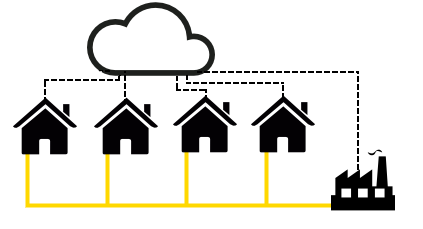
\includegraphics[width=0.7\textwidth]{billeder/CaseIlu.png}
\caption{Frequency comparison of the reconstruction methods}
\label{fig:CaseSetup}
\end{figure}

In the city setup is illustrated in figure \ref{fig:CaseSetup}. The figure is illustrated how the power company supplies power to the houses. All the houses have smart meters, and is informing the power company about the current consumption of each house, using some network. This is a fairly simplified example of a smart grid, that exists in many cities today. In this case it is assumed that the electric company receives information about the consumption of the houses each 30 seconds, as in the SmartHG dataset. Even though many smart meters today are capable of delivering information at this speed, it is more common to only get information each hour. This is mainly because the information is used to regulate distribution and production, which is a slow process that would not improve by faster update rates.  

The electric companies collect the information, and by using \ab{NILM} can calculate statistical information about the town. So if a TV station are making a analysis about the TV viewing habits in the town they are able to buy this information from the electric companies. 


\section{Results}





\section{Chapter Discussion}

